% !TeX program = xelatex
% Official ICLR 2026 style; course-project header replaces conference-status wording.
\documentclass[10pt,letterpaper]{article}
\usepackage{iclr2026_conference,times}
\usepackage{amsmath,amssymb,graphicx,booktabs,array,makecell,placeins}
\usepackage[hidelinks]{hyperref}
\iclrfinalcopy
\emergencystretch=1em
\newsavebox{\reporttablebox}
\usepackage{fontspec}
\setmainfont[Extension=.otf,UprightFont=*-regular,BoldFont=*-bold,ItalicFont=*-italic,BoldItalicFont=*-bolditalic]{texgyretermes}
\renewcommand{\sc}{\scshape}
\renewcommand{\bf}{\bfseries}
\renewcommand{\rm}{\rmfamily}
\title{\normalfont\scshape Routing Robustness in Mixture of Experts: Separating Expert Input and Routing Effects Across Perturbation Conditions}
\author{\begin{tabular}{ccc}
\textbf{Do Anh Dung} & \textbf{Yang Jian} & \textbf{Xiangli Qianhui}\\
\multicolumn{3}{c}{\normalfont Faculty of Information Science and Computing, University of Macau}\\
\normalfont\texttt{mc64468@um.edu.mo} & \normalfont\texttt{mc64796@um.edu.mo} & \normalfont\texttt{mc65432@um.edu.mo}
\end{tabular}}
\begin{document}
\maketitle
\lhead{CISC 7402 course project}


\begin{abstract}

Input perturbations can change both the predictions and expert selections of a mixture-of-experts model (MoE), but their simultaneous change does not establish that rerouting caused the prediction error. We ask how much of the error change comes from changes to expert inputs and how much comes from routing, and whether rerouting aggravates or compensates for input damage. We evaluate one trained model under four combinations of clean and perturbed expert inputs and routes. A forward path first changes the expert input and then the route, separating input and routing effects; a reverse path checks dependence on intervention order.


Across four synthetic regimes and seven joint-torque prediction tasks from SARCOS, noise-induced error increases are primarily attributed to expert-input effects on the forward path, with no clearly detected routing contribution. Removing the task cue increases both terms. Under feature masking, routing has a small effect on the synthetic tasks but partially compensates for input damage on SARCOS. Under some shortcut-feature shifts, input damage and routing compensation nearly cancel, so a small net error change conceals opposing internal effects. Routing-consistency training reduces expert switching but does not establish an additional accuracy gain over augmentation alone.


Within the tested conditions, the relative magnitude and direction of input and routing effects vary with the perturbation. Rerouting can either aggravate or mitigate prediction degradation. Assessing MoE robustness therefore requires comparing the two effects under a specified perturbation and intervention path, rather than treating expert-switch frequency as evidence that routing is harmful.


\end{abstract}

\FloatBarrier

\section{Introduction}

When an input perturbation changes both a mixture-of-experts prediction and its route, two mechanisms can contribute to the resulting error. The selected expert receives a different input, and the router may select a different expert or assign a different gate weight. An ordinary clean-versus-perturbed evaluation changes both at once. It therefore cannot determine which mechanism increased the error, or whether the route change actually reduced an otherwise larger input-induced error.


We study these mechanisms through paired interventions within one trained model. Holding the clean route fixed while changing the expert input measures an input effect. Allowing the route to change on that same perturbed input then measures a routing effect. A fourth evaluation reverses the order. The objective is to compare the effects under each perturbation condition, rather than assign one universal ranking to expert inputs and routing.


Our experiments distinguish changes to nuisance features, which preserve the predictive features and task cue, from masks and cue deletion, which remove predictive information. We use four controlled synthetic regimes and a real-data check on seven SARCOS torque-prediction tasks. Dense baselines contextualize prediction error and computational cost. Expert-removal tests assess specialization, and matched training arms test whether reducing route changes also improves accuracy.


The results show different mechanisms across conditions. On the forward path, nuisance-noise degradation is primarily an expert-input effect. Cue deletion makes both input and routing harmful. Synthetic feature masks have a small routing contribution, whereas SARCOS sensor masks induce beneficial rerouting. Some shortcut shifts produce opposing input and routing effects that nearly cancel. These comparisons motivate the secondary finding that routing stability and predictive robustness should be measured separately.


\begin{figure}[!htbp]

\centering

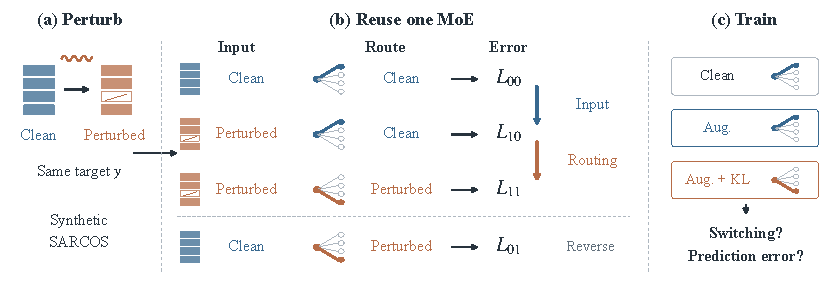
\includegraphics[width=\linewidth]{figures/figure1.pdf}

\caption{Paired intervention design. The same trained MoE is evaluated with four combinations of expert input and route. A route contains both expert identity and gate weight. Clean training, augmentation, and augmentation plus routing consistency provide a separate comparison of switching and prediction error.}

\label{fig:design1}

\end{figure}

\FloatBarrier

\section{Related Work}

Sparsely gated mixtures, GShard, Switch Transformers, ST-MoE, and V-MoE establish routing as a mechanism for conditional computation (\citealp{shazeer2017}; \citealp{lepikhin2021}; \citealp{fedus2022}; \citealp{zoph2022}; \citealp{riquelme2021}). BASE layers, hash layers, and expert-choice routing provide alternative allocation mechanisms (\citealp{lewis2021}; \citealp{roller2021}; \citealp{zhou2022}). Balance objectives can affect expert specialization (\citealp{chen2022}; \citealp{qiu2025}). \citet{puigcerver2022} examine connections between adversarial robustness, routing, and differences among experts.


Route-switch frequency and expert-load balance describe allocation, but neither directly measures the contribution of a route change to prediction error. Our paired four-cell contrasts, motivated by direct-effect and interchange decompositions (\citealp{pearl2001}; \citealp{geiger2021}), intervene on expert inputs and routes within a fixed model. The resulting contrasts are conditional on the selected intervention path. They do not identify a unique, order-independent allocation of error whenever input and route interact.


\FloatBarrier

\section{Experimental Design and Interventions}

\subsection{Synthetic tasks and training profiles}

Each synthetic input is $x=(e_c,u,v,m)$ in $\mathbb R^{28}$. The regime c belongs to \{1, 2, 3, 4\}; $e_{c}$ is its four-dimensional one-hot cue; u and v each have eight coordinates; and m is an eight-dimensional binary missingness indicator. Predictive features u are independent standard normal variables, independent of the regime. Before adding any shortcut offset, nuisance features v are also independent standard normals, independent of u and c.


The cue selects which of four functions generates the target. This changes the predictive map while holding the distribution of u fixed. Before regime-wise standardization, the functions are:


\[
f_1(u)=\frac{\sum_{i=1}^{8}u_i}{\sqrt{8}}
\]

\[
f_2(u)=\frac{\sum_{i=1}^{4}u_i-\sum_{i=5}^{8}u_i}{\sqrt{8}}
\]

\[
f_3(u)=\frac{u_1u_2+u_3u_4}{\sqrt{2}}
\]

\[
f_4(u)=\sin\left(\frac{\sum_{i=1}^{8}u_i}{\sqrt{8}}\right)
\]

The first two regimes are different linear directions; the third requires multiplicative interactions; the fourth applies a sine to the projection used by the first. Targets are $y=(f_c(u)-\mu_c)/\sigma_c$, with statistics computed on the training set. Standardization places the four regimes on a common MSE scale.


Training, validation, and test sets contain 80,000, 10,000, and 20,000 examples, balanced across regimes. Data-generation seeds are 10,000, 20,000, and 30,000. The same splits are shared by optimization seeds 0--4. Indicators remain zero during training. At mask evaluation, they either remain zero or mark missing coordinates.


The independent profile uses nuisance variables without a regime offset. The shortcut profile adds $2e_c$ to the first four nuisance coordinates during training and validation; test nuisance features have no offset. The explicit task cue remains visible in both profiles. Consequently, the shortcut-profile clean test condition already removes the training shortcut; later noise and shift interventions are paired with that clean test condition.


\subsection{Models and optimization}

The router is a 28 \ensuremath{\rightarrow} 128 \ensuremath{\rightarrow} 4 MLP with a Tanh hidden activation and a softmax output. Four experts are 28 \ensuremath{\rightarrow} 128 \ensuremath{\rightarrow} 128 \ensuremath{\rightarrow} 1 MLPs with ReLU hidden activations. The selected expert index is j(x), its softmax weight is w(x), and the prediction is $w(x)h_{j(x)}(x)$. Only the selected expert executes. The gate weight is retained rather than renormalized to one after top-1 selection.


Training minimizes MSE plus the balance loss $0.1\times4\sum_e F_e\bar p_e$, where $F_{e}$ is expert e's minibatch selection frequency and $\bar p_e$ its mean router probability. All models use 100 epochs, batch size 1,024, AdamW, constant learning rate 0.002, and weight decay $10^{-4}$. Checkpoints are selected by the lowest clean validation MSE.


The MoE has 85,640 parameters and 24,192 active linear multiply-accumulates (MACs) per example. The compute-matched dense network is 28 \ensuremath{\rightarrow} 139 \ensuremath{\rightarrow} 145 \ensuremath{\rightarrow} 1, with 24,477 parameters and 24,192 linear MACs. The parameter-matched network is 28 \ensuremath{\rightarrow} 206 \ensuremath{\rightarrow} 383 \ensuremath{\rightarrow} 1, with 85,639 parameters and 85,049 linear MACs. Both dense models use ReLU and the same optimization and checkpoint-selection rules. The MAC comparison counts linear operations and does not equate measured latency.


\subsection{Four-cell error decomposition}

Let $x_{0}$ be a clean input and $x_{1}$ its paired perturbation, with target y held fixed. A route is $g(x)=(j(x),w(x))$, containing expert identity and gate amplitude. Define:


\[
L_{ab}=\mathbb{E}[(F(x_a;g(x_b))-y)^2],\quad a,b\in\{0,1\}
\]

\[
F(x_a;g(x_b))=w(x_b)h_{j(x_b)}(x_a)
\]

$L_{00}$ is the clean evaluation and $L_{11}$ the ordinary perturbed evaluation. $L_{10}$ feeds the perturbed input to the expert selected by the clean route, with the clean gate weight. $L_{01}$ feeds the clean input using the perturbed route.


The forward path changes the expert input first and the route second:


\[
\Delta=L_{11}-L_{00}=A+R
\]

\[
A=L_{10}-L_{00},\qquad R=L_{11}-L_{10}
\]

A positive A indicates that changing the expert input increases error with the clean route fixed. A positive R indicates that adopting the perturbed route further increases error on that perturbed input; a negative R indicates compensation. Restoring the clean route on the perturbed input changes error by -R, so restoration helps when R is positive and hurts when R is negative.


The reverse path changes the route first. Its routing and input terms are $L_{01}$ - $L_{00}$ and $L_{11}$ - $L_{01}$. The interaction is:


\[
I=L_{11}-L_{10}-L_{01}+L_{00}
\]

\[
\mathrm{Reverse\ routing}=R-I,\quad\mathrm{Reverse\ input}=A+I
\]

When I is nonzero, the two orders allocate the same total differently. Throughout the results, ``Input'' and ``Routing'' denote forward-path effects unless stated otherwise. Input dominance on this path does not establish an order-independent ranking. These are within-model interventions, not claims that the clean route is optimal.


\subsection{Perturbations and uncertainty}

Nuisance perturbations are Gaussian noise $v'=v+\epsilon$, with epsilon distributed as $\mathcal N(0,s^2I_8)$, and mean shifts $v'_i=v_i+s$ on all eight nuisance coordinates, at $s=0.25,0.5,1$. Predictive features and the cue remain intact. Information-loss tests uniformly mask one, two, or four predictive coordinates by replacing them with zero, or zero the task cue on 25\%, 50\%, or 75\% of items. Mask indicators are either left zero or activated at test. Targets stay fixed.


Switch rate is the fraction of paired items whose top-1 expert changes. Gate entropy is mean Shannon entropy in nats, with maximum log(4) \ensuremath{\approx} 1.386. Maximum load is the largest expert selection frequency on a test set. Identity-only controls hold the perturbed gate weight fixed while restoring the clean expert index.


Stochastic perturbations use three matched draws averaged within source item; mean shifts are deterministic. For each fixed data split, percentile 95\% intervals use 1,000 paired crossed-bootstrap resamples of training-seed IDs and source-item IDs. Sampled sources are shared across seeds and model comparisons. An interval containing zero indicates that the comparison does not establish a directional effect; it does not demonstrate equivalence or an exactly zero effect.


\FloatBarrier

\section{Expert Specialization as a Diagnostic}

On the independent profile, the dominant expert receives, on average, 0.579 of a regime's clean routes. Removing that expert reroutes to the highest remaining router probability while retaining the original selected weight. This increases MSE by 0.326, with interval [0.089, 0.694]. Forcing one of the other three experts, averaged over regimes and seeds and retaining the same gate weight, yields MSE 1.310. These interventions indicate that experts are not interchangeable. Expert labels are seed-specific and should not be aligned across seeds without further matching.


\begin{figure}[!htbp]

\centering

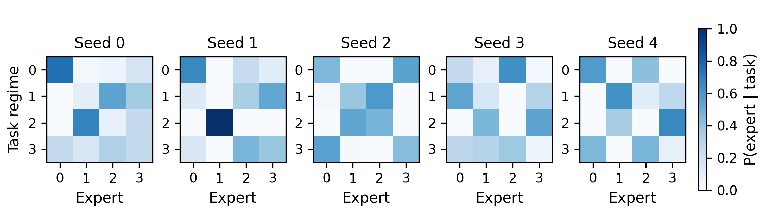
\includegraphics[width=\linewidth]{figures/figure2.pdf}

\caption{Per-seed routing matrices on the independent profile. Expert columns are specific to each training seed.}

\label{fig:design2}

\end{figure}

Across the 20 seed-regime pairs, the Pearson correlation between dominant-expert removal cost and total perturbation-induced MSE change is 0.11 for noise at scale 1, 0.10 for mean shift at scale 1, 0.41 for a 25\% predictive mask with indicators off, and -0.33 for cue removal on 50\% of items. These are descriptive associations. Removal cost is substantial, but its relationship with noise and shift degradation is weak. Specialization therefore does not replace a direct comparison of input and routing effects in each perturbation condition.


\FloatBarrier

\section{Perturbations That Preserve Predictive Information}

Noise and shifts act on nuisance coordinates while retaining predictive features and the task cue. They test whether error can increase without deleting task information, and whether rerouting contributes to that increase. Table 1 reports absolute MSE. Table 2 reports changes relative to the paired clean evaluation, multiplied by 10,000 for readability. Thus, 1.49 in Table 2 means a change of 0.000149, whereas 0.000838 in Table 1 is an unscaled error level.


\begin{table}[!htbp]
\centering
\caption{Absolute test MSE averaged over five training seeds. Noise and shift scales are 1. Masking removes 25\% of predictive coordinates with indicators off; cue removal affects 50\% of items. Test nuisance features have no shortcut offset before perturbation. MAC and Param identify compute-matched and parameter-matched dense networks.}
\label{tab:results1}
\small
\setlength{\tabcolsep}{4pt}
\renewcommand{\arraystretch}{1.1}
\sbox{\reporttablebox}{%
\begin{tabular}{@{}llrrr@{}}
\toprule
Profile & Condition & MoE & Dense MAC & Dense Param \\
\midrule
Independent & Clean & 0.000698 & 0.000636 & 0.000540 \\
Independent & Noise & 0.000838 & 0.000690 & 0.000596 \\
Independent & Shift & 0.000849 & 0.000671 & 0.000610 \\
Independent & Mask 25\% & 0.322864 & 0.322765 & 0.322870 \\
Independent & Cue removal 50\% & 0.432599 & 0.400901 & 0.349836 \\
Shortcut & Clean & 0.000748 & 0.000840 & 0.000758 \\
Shortcut & Noise & 0.001262 & 0.001075 & 0.000955 \\
Shortcut & Shift & 0.000751 & 0.000802 & 0.000813 \\
Shortcut & Mask 25\% & 0.322852 & 0.323029 & 0.322856 \\
Shortcut & Cue removal 50\% & 0.475609 & 0.383032 & 0.349046 \\
\bottomrule
\end{tabular}}
\ifdim\wd\reporttablebox>\linewidth
\resizebox{\linewidth}{!}{\usebox{\reporttablebox}}
\else\usebox{\reporttablebox}\fi
\end{table}


\subsection{Independent profile}

Across the tested noise and shift scales, the forward input term is positive and its interval excludes zero. Forward routing terms are smaller and all their intervals contain zero. At noise scale 1, the input and routing effects are 1.49 and -0.10 in Table 2 units. This supports input dominance on the forward path, without establishing that routing has exactly no effect.


Expert switching nevertheless increases with perturbation scale: from 0.0057 to 0.0235 under noise and from 0.0072 to 0.0274 under mean shifts. Maximum load remains between 0.254 and 0.258. Switching is observable even when its forward-path contribution to prediction error is not clearly detected.


\begin{table}[!htbp]
\centering
\caption{Forward decomposition under nuisance perturbations. Every numeric effect and interval endpoint is a change in MSE multiplied by 10,000. Brackets are paired 95\% intervals. A is Input, R is Routing, and I is interaction.}
\label{tab:results2}
\small
\setlength{\tabcolsep}{4pt}
\renewcommand{\arraystretch}{1.1}
\sbox{\reporttablebox}{%
\begin{tabular}{@{}llrrrr@{}}
\toprule
Profile and test & Scale & Input A & Routing R & Interaction I & Total \\
\midrule
\makecell[l]{Independent\\noise} & 0.25 & \makecell[r]{0.07\\{}[0.04, 0.10]} & \makecell[r]{0.01\\{}[-0.03, 0.05]} & \makecell[r]{-0.05\\{}[-0.08, -0.03]} & \makecell[r]{0.08\\{}[0.04, 0.13]} \\
\makecell[l]{Independent\\noise} & 0.50 & \makecell[r]{0.34\\{}[0.23, 0.49]} & \makecell[r]{-0.04\\{}[-0.15, 0.05]} & \makecell[r]{-0.19\\{}[-0.30, -0.12]} & \makecell[r]{0.30\\{}[0.18, 0.49]} \\
\makecell[l]{Independent\\noise} & 1 & \makecell[r]{1.49\\{}[1.02, 2.10]} & \makecell[r]{-0.10\\{}[-0.41, 0.13]} & \makecell[r]{-0.88\\{}[-1.43, -0.51]} & \makecell[r]{1.40\\{}[0.91, 1.95]} \\
\makecell[l]{Independent\\shift} & 0.25 & \makecell[r]{0.11\\{}[0.05, 0.19]} & \makecell[r]{-0.02\\{}[-0.11, 0.11]} & \makecell[r]{-0.05\\{}[-0.08, -0.03]} & \makecell[r]{0.10\\{}[-0.03, 0.22]} \\
\makecell[l]{Independent\\shift} & 0.50 & \makecell[r]{0.40\\{}[0.25, 0.55]} & \makecell[r]{-0.03\\{}[-0.20, 0.17]} & \makecell[r]{-0.19\\{}[-0.27, -0.12]} & \makecell[r]{0.37\\{}[0.10, 0.64]} \\
\makecell[l]{Independent\\shift} & 1 & \makecell[r]{1.60\\{}[1.14, 2.13]} & \makecell[r]{-0.10\\{}[-0.42, 0.32]} & \makecell[r]{-0.69\\{}[-1.00, -0.37]} & \makecell[r]{1.50\\{}[0.85, 2.40]} \\
\midrule
\makecell[l]{Shortcut\\noise} & 0.25 & \makecell[r]{0.24\\{}[0.15, 0.34]} & \makecell[r]{-0.04\\{}[-0.11, 0.02]} & \makecell[r]{-0.17\\{}[-0.25, -0.11]} & \makecell[r]{0.20\\{}[0.09, 0.32]} \\
\makecell[l]{Shortcut\\noise} & 0.50 & \makecell[r]{1.15\\{}[0.92, 1.51]} & \makecell[r]{-0.11\\{}[-0.42, 0.26]} & \makecell[r]{-0.68\\{}[-1.03, -0.41]} & \makecell[r]{1.04\\{}[0.69, 1.57]} \\
\makecell[l]{Shortcut\\noise} & 1 & \makecell[r]{5.31\\{}[4.32, 6.31]} & \makecell[r]{-0.17\\{}[-1.49, 1.18]} & \makecell[r]{-2.55\\{}[-4.14, -1.38]} & \makecell[r]{5.14\\{}[3.68, 6.83]} \\
\makecell[l]{Shortcut\\shift} & 0.25 & \makecell[r]{-0.16\\{}[-0.46, 0.07]} & \makecell[r]{-0.24\\{}[-0.38, -0.14]} & \makecell[r]{-0.25\\{}[-0.58, -0.06]} & \makecell[r]{-0.40\\{}[-0.73, -0.21]} \\
\makecell[l]{Shortcut\\shift} & 0.50 & \makecell[r]{0.20\\{}[-0.36, 0.95]} & \makecell[r]{-0.68\\{}[-1.26, -0.28]} & \makecell[r]{-1.00\\{}[-2.25, -0.21]} & \makecell[r]{-0.48\\{}[-0.84, -0.20]} \\
\makecell[l]{Shortcut\\shift} & 1 & \makecell[r]{2.33\\{}[0.51, 5.13]} & \makecell[r]{-2.29\\{}[-4.88, -0.61]} & \makecell[r]{-3.93\\{}[-8.78, -0.82]} & \makecell[r]{0.04\\{}[-0.47, 0.53]} \\
\bottomrule
\end{tabular}}
\ifdim\wd\reporttablebox>\linewidth
\resizebox{\linewidth}{!}{\usebox{\reporttablebox}}
\else\usebox{\reporttablebox}\fi
\end{table}


\subsection{Shortcut profile and compensation}

On shortcut-trained models, noise produces larger forward input effects, while routing intervals again contain zero. Mean shifts produce a different mechanism: R is negative at every tested scale, with intervals below zero. The perturbed route therefore reduces error relative to retaining the clean route on the shifted input.


At scales 0.25 and 0.5, total error changes are negative and input-effect intervals contain zero. At scale 1, the input effect is +2.33 [0.51, 5.13] and the routing effect is -2.29 [-4.88, -0.61], in Table 2 units. The total is 0.04 [-0.47, 0.53]. A small net change here reflects nearly offsetting input damage and routing compensation, rather than an absence of internal effects. Switch rates range from 0.0067 to 0.0263 and maximum load from 0.258 to 0.262.


Removing the shortcut offset itself, while preserving the target and cue, increases MoE MSE by 0.000301 [0.000181, 0.000543]. The corresponding compute-matched dense increase is 0.000217 [0.000147, 0.000311]. These offset-removal comparisons are distinct from the additional shifts in Table 2.


\subsection{Reverse path and attribution limits}

Table 3 reports the reverse path in raw MSE. On the independent profile, its routing and input terms are both below 0.0001, but this does not imply the same relative attribution as the forward path. For noise at scale 1, the route-first contribution is 0.000078 out of a total change of approximately 0.000140. The contrast demonstrates that a small forward routing term can coexist with a larger reverse routing term.


\begin{table}[!htbp]
\centering
\caption{Reverse-path means at scale 1, in raw MSE. The routing term changes the route on clean expert input; the input term then changes the expert input under that route.}
\label{tab:results3}
\small
\setlength{\tabcolsep}{4pt}
\renewcommand{\arraystretch}{1.1}
\sbox{\reporttablebox}{%
\begin{tabular}{@{}llrr@{}}
\toprule
Profile & Family & Route first $L_{01}$ - $L_{00}$ & Input second $L_{11}$ - $L_{01}$ \\
\midrule
Independent & Noise & 0.000078 & 0.000062 \\
Independent & Shift & 0.000059 & 0.000091 \\
Shortcut & Noise & 0.000238 & 0.000276 \\
Shortcut & Shift & 0.000164 & -0.000160 \\
\bottomrule
\end{tabular}}
\ifdim\wd\reporttablebox>\linewidth
\resizebox{\linewidth}{!}{\usebox{\reporttablebox}}
\else\usebox{\reporttablebox}\fi
\end{table}


For the shortcut shift, changing the route on clean expert input increases MSE by 0.000164. Changing the expert input afterwards lowers it by 0.000160. At scales 0.25 and 0.5, the second term is -0.000042 and -0.000081. The shifted route is beneficial when paired with the shifted expert input, not when transplanted onto the clean input. Accordingly, the forward and reverse paths describe different conditional effects; neither supports a universal ranking of routing and input importance.


\subsection{Dense baselines and measured cost}

Under 25\% masking, the three architectures have nearly identical mean errors. Under cue removal, the MoE has higher mean MSE than both dense baselines in both profiles. At independent-profile noise scale 1, the paired MoE-minus-dense differences are 0.000148 [-0.000200, 0.000412] for the compute-matched model and 0.000242 [-0.000082, 0.000503] for the parameter-matched model. These intervals do not establish a difference.


On one A800 at batch size 1,024, clean-input latency is 1.193 ms for the MoE with Python expert dispatch, 0.144 ms for the compute-matched dense model, and 0.145 ms for the parameter-matched model. Measurements are medians of 30 synchronized forwards after 10 warm-ups. Matching active linear MACs does not match latency in this implementation.


\FloatBarrier

\section{Feature Masks and Task Cue Removal}

Masks remove predictive coordinates while leaving the task cue intact. Cue deletion removes the variable that identifies which predictive map is required. Both remove information, but they need not produce the same routing effect.


\subsection{Irreducible error under synthetic masks}

Let k of eight predictive coordinates be masked, $q=k/8$, and O contain the observed coordinates, mask locations, and cue. For any predictor h(O):


\[
\mathbb{E}[(Y-h(O))^2]=\mathbb{E}[\mathrm{Var}(Y\mid O)]+\mathbb{E}[(\mathbb{E}[Y\mid O]-h(O))^2]
\]

The first term is a reference risk due to unavailable information; the second is excess prediction error above that reference. For the two linear regimes, raw reference risk is q. For the product regime, averaged over uniformly selected mask locations, it is $1-(8-k)(7-k)/56$. For the sine regime, with $S_{o}$ the observed normalized sum, the conditional mean is $e^{-q/2}\sin(S_o)$, and raw reference risk is:


\[
\frac{1-e^{-2}-e^{-q}+e^{-2+q}}{2}
\]

Each regime's risk is divided by its training target variance. This reference-risk calculation is separate from the four-cell decomposition: Tables 4 and 5 split the change $L_{11}$ - $L_{00}$, not the model's excess over the reference risk.


\subsection{Synthetic masking}

On the independent profile, as the mask increases from one to four coordinates, the total MSE increase grows from approximately 0.167 to 0.596. Forward input terms are 0.160, 0.313, and 0.588, whereas routing terms remain below 0.01. Switching rises from 0.121 to 0.272 and maximum load remains between 0.256 and 0.264. Thus, substantial switching can accompany an input-dominated forward decomposition. The shortcut profile shows the same broad pattern, with somewhat larger routing terms.


\begin{table}[!htbp]
\centering
\caption{Shortcut-profile information-loss effects. Input, Routing, and Total are changes in raw MSE; Switch is an expert-ID switch rate. Mask indicators remain zero.}
\label{tab:results4}
\small
\setlength{\tabcolsep}{4pt}
\renewcommand{\arraystretch}{1.1}
\sbox{\reporttablebox}{%
\begin{tabular}{@{}llrrrr@{}}
\toprule
Family & Level & Input & Routing & Total & Switch \\
\midrule
Mask & 12.5\% & 0.160 & 0.0069 & 0.167 & 0.114 \\
Mask & 25\% & 0.311 & 0.0113 & 0.322 & 0.163 \\
Mask & 50\% & 0.581 & 0.0155 & 0.596 & 0.238 \\
Cue removal & 25\% & 0.127 & 0.107 & 0.234 & 0.166 \\
Cue removal & 50\% & 0.259 & 0.215 & 0.475 & 0.332 \\
Cue removal & 75\% & 0.389 & 0.333 & 0.722 & 0.499 \\
\bottomrule
\end{tabular}}
\ifdim\wd\reporttablebox>\linewidth
\resizebox{\linewidth}{!}{\usebox{\reporttablebox}}
\else\usebox{\reporttablebox}\fi
\end{table}


At independent-profile 25\% masking, the identity-only restoration benefit is -0.0034 [-0.0067, 0.0003], where positive means lower MSE after restoring the clean expert identity at the perturbed weight. Restoring the identity therefore does not establish a repair in this condition.


The marker control compares identical masks with indicators off and on. With indicators off at 25\% masking, this paired control gives MoE MSE 0.322395 and an empirical conditional-mean reference MSE of 0.319043; the excess is 0.003352 [0.002758, 0.003912]. Table~\ref{tab:results1} instead reports 0.322864 from the original stand-alone mask-without-indicators evaluation. Both evaluations reuse the same checkpoints and test sources, but use different mask draws: seeds 9015--9017 for the paired control and 9024--9026 for the stand-alone condition. Their absolute MSEs therefore need not coincide. Activating indicators only at test, after training with indicators always zero, adds error: 0.0108 [0.0082, 0.0135] at 12.5\%, 0.0185 [0.0136, 0.0238] at 25\%, and 0.0261 [0.0197, 0.0325] at 50\%. These comparisons test a training--evaluation mismatch, not the value of indicators learned during training. At 25\% masking with indicators activated, MoE-minus-compute-matched-dense MSE is -0.0231 [-0.0461, -0.0092].


\begin{table}[!htbp]
\centering
\caption{Independent-profile information-loss effects. Effects are changes in raw MSE. Mask indicators remain zero.}
\label{tab:results5}
\small
\setlength{\tabcolsep}{4pt}
\renewcommand{\arraystretch}{1.1}
\sbox{\reporttablebox}{%
\begin{tabular}{@{}llrrrr@{}}
\toprule
Family & Level & Input & Routing & Total & Switch \\
\midrule
Mask & 12.5\% & 0.160 & 0.0067 & 0.167 & 0.121 \\
Mask & 25\% & 0.313 & 0.0093 & 0.322 & 0.182 \\
Mask & 50\% & 0.588 & 0.0078 & 0.596 & 0.272 \\
Cue removal & 25\% & 0.138 & 0.074 & 0.212 & 0.149 \\
Cue removal & 50\% & 0.283 & 0.149 & 0.432 & 0.298 \\
Cue removal & 75\% & 0.425 & 0.228 & 0.653 & 0.444 \\
\bottomrule
\end{tabular}}
\ifdim\wd\reporttablebox>\linewidth
\resizebox{\linewidth}{!}{\usebox{\reporttablebox}}
\else\usebox{\reporttablebox}\fi
\end{table}


\subsection{Cue removal}

Cue deletion increases both forward terms. On the independent profile, switching rises from 0.149 to 0.444 as cue removal increases from 25\% to 75\% of items. At 50\%, the input term is 0.283 [0.248, 0.321] and the routing term is 0.149 [0.086, 0.208]. Restoring the clean route on the perturbed input therefore reduces error in this condition. The identity-only restoration benefit is 0.176 [0.105, 0.247], supporting an important expert-selection contribution, without establishing that gate amplitude has no role. Maximum load increases from 0.307 to 0.436 across cue-removal rates.


The shortcut profile also has positive input and routing terms. At 50\% cue removal they are 0.259 and 0.215. Input remains the larger mean contribution, but routing accounts for a greater share than on the independent profile. Unlike masking, cue deletion makes the route change itself harmful on the forward path.


Clean gate entropy is already high: 1.267 for the independent profile and 1.303 for the shortcut profile, against log(4) \ensuremath{\approx} 1.386. Noise, shifts, and zero-indicator masks change it by less than 0.003. At 75\% cue deletion it rises to 1.329 [1.311, 1.347] and 1.358 [1.352, 1.364], respectively. Entropy and load characterize the routing response, while the intervention contrasts determine whether that response increases error.


\FloatBarrier

\section{Routing Consistency as a Secondary Training Test}

The preceding sections compare the effects of input and routing changes under fixed checkpoints. We next test whether explicitly reducing routing changes produces a detectable prediction benefit. Each profile has three arms: clean training, nuisance-noise augmentation at SD 0.5, and augmentation plus $0.1D_{\mathrm{KL}}(\operatorname{stopgrad}(p(x))\Vert p(\tilde x))$, where p is the router softmax.


Augmentation and consistency arms average clean-view and noisy-view MSE and balance losses. The clean arm uses two identical clean views. Arms share per-seed initialization, minibatch order, and matched noise draws where applicable, and use the same 100-epoch schedule and clean-validation checkpoint rule. The clean controls are trained anew for this matched comparison, so they differ from Table 1.


\begin{table}[!htbp]
\centering
\caption{Matched synthetic training comparison at perturbation scale 1. MSE values are absolute, unscaled errors; switch values are expert-ID switch rates. The final column is consistency minus augmentation MSE.}
\label{tab:results6}
\small
\setlength{\tabcolsep}{4pt}
\renewcommand{\arraystretch}{1.1}
\sbox{\reporttablebox}{%
\begin{tabular}{@{}llrrrr@{}}
\toprule
Profile & Test and metric & Clean & Augmentation & Consistency & Cons. - Aug. \\
\midrule
Independent & Noise MSE & 0.000899 & 0.000787 & 0.000669 & -0.000118 \\
Independent & Noise switch & 0.0288 & 0.0230 & 0.0160 & --- \\
Independent & Shift MSE & 0.000897 & 0.000731 & 0.000674 & -0.000057 \\
Independent & Shift switch & 0.0318 & 0.0311 & 0.0153 & --- \\
Shortcut & Noise MSE & 0.001392 & 0.000868 & 0.000598 & -0.000270 \\
Shortcut & Noise switch & 0.0400 & 0.0315 & 0.0109 & --- \\
Shortcut & Shift MSE & 0.000782 & 0.000705 & 0.000440 & -0.000264 \\
Shortcut & Shift switch & 0.0409 & 0.0256 & 0.0099 & --- \\
\bottomrule
\end{tabular}}
\ifdim\wd\reporttablebox>\linewidth
\resizebox{\linewidth}{!}{\usebox{\reporttablebox}}
\else\usebox{\reporttablebox}\fi
\end{table}


Augmentation lowers mean error relative to clean training. Consistency has the lowest mean error and switch rate in all four scale-1 comparisons. However, the paired consistency-minus-augmentation MSE intervals all contain zero: [-0.000299, 0.000043] and [-0.000254, 0.000112] for independent-profile noise and shift, and [-0.000748, 0.000023] and [-0.000641, 0.000004] for shortcut-profile noise and shift. The results show lower observed switching, but do not establish an additional accuracy gain over augmentation. They also do not establish equivalence between the two methods.


\begin{figure}[!htbp]

\centering

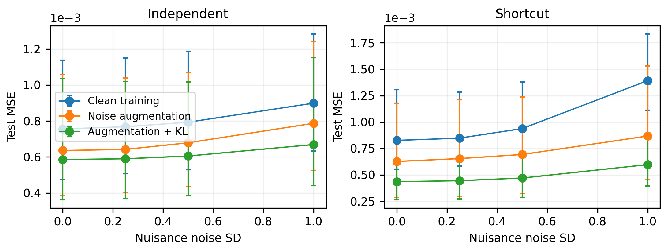
\includegraphics[width=\linewidth]{figures/figure3.pdf}

\caption{Synthetic nuisance-noise response of the matched training arms. Error bars show 95\% intervals for arm means. Paired error-difference intervals are reported in the text.}

\label{fig:design3}

\end{figure}

\subsection{Separating expert identity and gate amplitude}

A route contains two components, so restoring it may combine effects of opposite signs. Hold the noise-SD-1 expert input z fixed and define:


\[
M_{ab}=\mathbb{E}[(w_b h_{j_a}(z)-y)^2]
\]

\[
(j_0,w_0)=g(x),\qquad(j_1,w_1)=g(z)
\]

\[
B_{\mathrm{ID}}=M_{11}-M_{01},\quad B_w=M_{11}-M_{10},\quad B_{\mathrm{joint}}=M_{11}-M_{00}
\]

Positive B denotes a reduction in MSE after restoration. These cells share checkpoints, inputs, and three noise draws. On the shortcut augmentation arm, restoring the clean expert identity reduces error, with benefit 4.23 \ensuremath{\times} $10^{-5}$ [0.82, 8.99] \ensuremath{\times} $10^{-5}$. Restoring the clean gate weight increases error, with benefit -5.65 \ensuremath{\times} $10^{-5}$ [-8.72, -2.68] \ensuremath{\times} $10^{-5}$. Joint restoration has benefit -1.51 \ensuremath{\times} $10^{-5}$ [-6.14, 3.61] \ensuremath{\times} $10^{-5}$. Thus, identity restoration is beneficial and weight restoration harmful in this condition, while the joint effect is not clearly separated from zero. These conditional benefits need not add because identity and weight can interact.


All four experts remain active in the 30 checkpoints. Mean maximum load ranges from 0.258 to 0.277 across the six profile-arm combinations, and the largest individual load is 0.312. No arm concentrates all selections on one expert.


\FloatBarrier

\section{Real Data Validation on SARCOS}

\subsection{Task and evaluation design}

SARCOS inverse dynamics provides 21 sensor coordinates, comprising position, velocity, and acceleration for each of seven joints, and seven torque targets (\citealp{vijayakumar2005}). We predict one joint torque at a time and place a seven-dimensional one-hot joint cue before the 21 sensor coordinates. This yields 28 input dimensions, allowing reuse of the synthetic architectures. The added cue identifies the prediction task; it is not an original sensor variable in the archive.


Removing 4,428 development records with input states identical to test states leaves 35,056 training, 5,000 validation, and 4,449 test records, using split seed 20261027. Input scaling and per-joint target standardization use only training data. Each epoch assigns one joint per training source, cycling through all seven joints every seven epochs. Validation and test cover all joints.


Seven configurations across optimization seeds 0--4 yield 35 runs: clean and augmented versions of all three architectures, plus MoE augmentation with consistency. Optimization follows Section 3.2. Seeds share source order and joint assignments across configurations, with shared initialization within each architecture. Augmentation adds SD-0.1 noise to standardized sensor coordinates; the consistency coefficient is 0.1.


Tests add sensor-noise SDs 0.1, 0.25, and 0.5, uniformly zero three or six sensor coordinates, or remove the joint cue on 50\% of sources. Targets remain fixed. Each source shares its corrupted state across joint tasks. Macro-NMSE averages training-variance-normalized squared error over joints and sources. Three perturbation draws and seven joints are averaged within source before the crossed bootstrap. The primary endpoint is consistency minus augmentation at noise SD 0.25.


SARCOS sensor perturbations affect features used to predict torque, whereas synthetic nuisance noise leaves the predictive coordinates intact. Their error magnitudes should therefore not be compared as if the perturbations had identical meanings. Table 7 reports unscaled absolute macro-NMSE, not the scaled changes in Table 2.


\begin{table}[!htbp]
\centering
\caption{SARCOS macro-NMSE averaged over five seeds. Noise has SD 0.25; masking removes six of 21 sensor coordinates. Switch is the expert-ID switch rate at noise SD 0.25.}
\label{tab:results7}
\small
\setlength{\tabcolsep}{4pt}
\renewcommand{\arraystretch}{1.1}
\sbox{\reporttablebox}{%
\begin{tabular}{@{}llrrrr@{}}
\toprule
Model & Training & Clean & Noise 0.25 & Mask 6/21 & Switch \\
\midrule
MoE & Clean & 0.016179 & 0.114362 & 0.409034 & 0.0669 \\
Dense MAC & Clean & 0.018466 & 0.124025 & 0.441438 & --- \\
Dense Param & Clean & 0.015070 & 0.117297 & 0.434594 & --- \\
MoE & Augmentation & 0.017630 & 0.075124 & 0.307793 & 0.0660 \\
Dense MAC & Augmentation & 0.019639 & 0.085397 & 0.339033 & --- \\
Dense Param & Augmentation & 0.015967 & 0.075076 & 0.318832 & --- \\
MoE & Augmentation + KL & 0.017667 & 0.075180 & 0.306018 & 0.0609 \\
\bottomrule
\end{tabular}}
\ifdim\wd\reporttablebox>\linewidth
\resizebox{\linewidth}{!}{\usebox{\reporttablebox}}
\else\usebox{\reporttablebox}\fi
\end{table}


\subsection{Input damage and routing compensation}

At noise SD 0.25, the clean-trained MoE has forward input effect 0.097793 [0.094766, 0.100639] and routing effect 0.000390 [-0.000661, 0.001534]. The total change is therefore overwhelmingly attributed to the input term on this path. A switch rate of 0.0669 coexists with no clearly detected forward routing contribution.


Six-coordinate masking differs from synthetic masking. The input term is 0.425050, while the routing term is -0.032195 [-0.043868, -0.020455]. Rerouting partially offsets the input-induced error, although it does not eliminate the degradation. Restoring the clean route would increase error relative to allowing the model to reroute. Cue removal instead produces positive input and routing terms, 0.390242 and 0.016638, respectively. Their mean directions match the synthetic cue-removal results; no interval for the SARCOS cue-routing term is reported here.


\begin{figure}[!htbp]

\centering

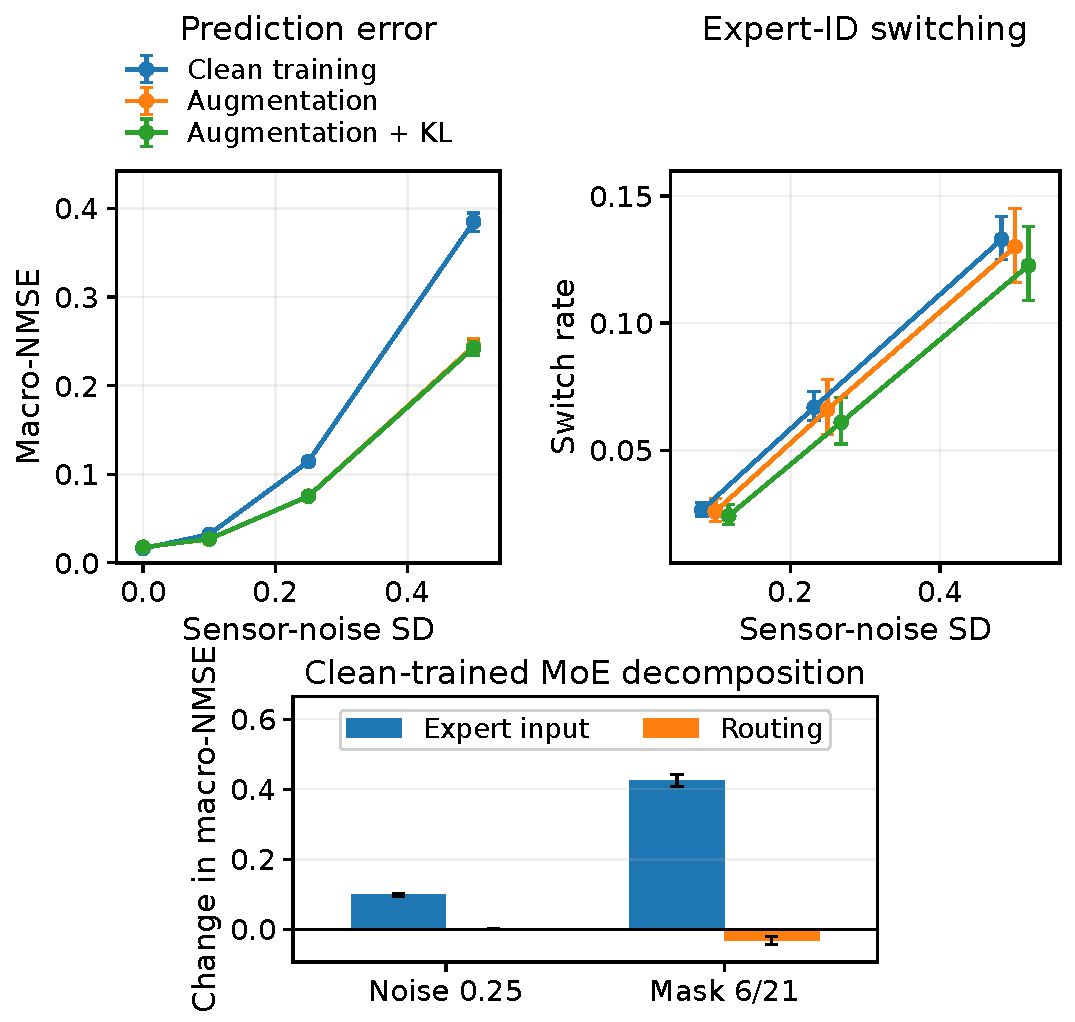
\includegraphics[width=\linewidth]{figures/figure4.pdf}

\caption{SARCOS noise-response curves for the three MoE training arms and the clean-trained MoE's forward-path decomposition. Error bars are 95\% crossed-bootstrap intervals.}

\label{fig:design4}

\end{figure}

\subsection{Training comparison}

Augmentation lowers MoE mean macro-NMSE at noise SD 0.25 from 0.114362 to 0.075124. Adding consistency changes it to 0.075180. The paired consistency-minus-augmentation difference is 0.000056 [-0.000928, 0.001403], so no additional error reduction is established at the primary endpoint.


Switching falls from 0.0660 to 0.0609, a paired difference of -0.005071 [-0.008952, -0.001401]. Under six-coordinate masking, the prediction-error difference is -0.001774 [-0.005062, 0.001536], again including zero. All four experts remain active in each MoE checkpoint. SARCOS therefore supports the separation between a detected reduction in switching and an unestablished additional accuracy benefit.


\FloatBarrier

\section{Limitations}

The synthetic regimes are hand-specified and provide the task cue explicitly. Their specialization problem is easier than discovering task boundaries from raw inputs. The SARCOS joint cue is also added by the experiment. SARCOS extends the evaluation beyond the synthetic target functions, but does not remove dependence on an explicit task identifier.


The models are small top-1 mixtures with four MLP experts and a retained scalar softmax gate. Results do not establish the behavior of sparse language or vision models, top-k routing, expert-choice routing, or other gate conventions. Dense comparisons use networks from the same feed-forward family, and measured dispatch cost is implementation-specific.


Synthetic nuisance effects are often of order $10^{-4}$ against absolute MSE near $10^{-3}$. Some estimated directions are supported by intervals, but the practical error changes remain small. Five seeds, one model scale, and fixed data splits limit inference. Intervals containing zero do not prove absence of an effect, equivalence, or a lack of possible benefit from consistency training.


The decomposition is path-dependent whenever interaction is nonzero. A forward input-dominated result may coexist with a larger route-first contribution. The route contrasts also combine expert identity and gate amplitude unless they are explicitly separated. Consequently, ``input effect'' and ``routing effect'' must always be read with their intervention definitions.


Perturbations are isotropic noise, constant mean shifts, random coordinate masks, and cue deletion. They are not adversarial, and apart from SARCOS coordinate masks are not designed to model a specific sensor failure. Targets stay fixed; this is an evaluation of prediction under corrupted observations, not a simulation of how physical targets change when the underlying state changes.


SARCOS is one arm and one archive. After removing development records whose inputs exactly match test inputs, source records are treated as independent. Dependence along original trajectories is ignored. Averaging within source addresses shared joint tasks and perturbation draws, but does not account for dependence between different trajectory records.


\FloatBarrier

\section{Discussion and Conclusion}

This study asks how perturbation-induced error changes are divided between expert inputs and routing, and whether the route change worsens or mitigates the damage. The answer varies across the tested perturbation conditions. On the specified forward path, noise degradation is primarily an input effect in both synthetic experiments and SARCOS, with no clearly detected routing contribution. Deleting the task cue increases both terms. Synthetic masks are input-dominated, whereas SARCOS sensor masks produce beneficial rerouting. Under the largest shortcut shift, input damage and routing compensation nearly cancel.


These results do not provide a universal ranking of the two mechanisms. They show why the comparison must specify what was perturbed and which intervention path was used. A small net error change may conceal opposing effects, and a high switch rate may accompany harmful, negligible, or beneficial routing contributions. Conversely, restoring a clean route is condition-dependent: it lowers error under cue removal, but increases error under the shortcut shifts and SARCOS masks where the perturbed route provides compensation.


Expert specialization and routing consistency provide supporting diagnostics rather than substitutes for this decomposition. Dominant-expert removal is costly but only weakly associated with noise and shift degradation. Consistency training lowers observed synthetic switching and produces a detected switching reduction at the primary SARCOS condition, while its paired error intervals do not establish an additional accuracy gain over augmentation. Separating expert identity and gate amplitude further reveals that restoring one component can help while restoring the other hurts.


Within the tested conditions, the relative magnitude and direction of input and routing effects depend on the perturbation. Rerouting can aggravate or mitigate prediction degradation. MoE robustness should therefore be assessed by directly comparing the two effects under specified perturbations and interventions, rather than inferring routing damage from expert-switch frequency alone.


\FloatBarrier

\section*{Contributions}

Do Anh Dung built the tasks, perturbations, shortcut profile, and four-cell interventions. Yang Jian built the MoE and dense models, multi-seed training, and measurement pipeline. Xiangli Qianhui computed the decomposition, bootstrap intervals, route summaries, and report. AI tools assisted literature search, implementation, and drafting.


\FloatBarrier

\nocite{*}

\bibliographystyle{iclr2026_conference}

\bibliography{references}

\end{document}